\documentclass[12pt,a4paper,UTF8,AutoFakeBold]{ctexbook} %注意AutoFackBold打开用来加粗中文字体

\usepackage{xcolor}
\usepackage{xeCJK}
\usepackage{graphicx}
\usepackage{amsmath}
\usepackage{ctexcap}
\usepackage{fancyhdr}
\usepackage{caption2}
\usepackage[ colorlinks=true, linkcolor=blue]{hyperref}

%图标题设置
\renewcommand{\captionfont}{\songti\zihao{5}} %图标题5号
\setlength{\textfloatsep} {0pt} %设置图与下文的距离:http://bbs.ctex.org/forum.php?mod=viewthread&tid=70899
\captionsetup{format=hang, aboveskip=0pt, belowskip=0pt}
\setlength{\floatsep}{0pt} %图片间的距离 http://www.ctex.org/documents/latex/graphics/node72.html
%插入图片的命令
\newcommand{\myfig}[4]{%#1标题 #2label #3宽度 #4img_path
		\begin{figure}[!ht]
		\begin{center}
			\setlength{\belowcaptionskip}{10pt}
			\includegraphics[width=#3\textwidth]{#4}
			\caption{#1}\label{#2}
		\end{center}
	\end{figure}
}
%引用学习 http://www.latexstudio.net/archives/3297
%http://blog.sina.com.cn/s/blog_7101508c0100tgg4.html
%页眉面脚 参见《latex2e完全学习手册》4.4版式 页眉与页脚
\pagestyle{fancy}
\fancyhead[EL,OL,ER,OR]{}
\fancyhead[EC]{西安电子科技大学}
\fancyhead[OC]{\leftmark}
\fancyfoot[C]{\thepage}

\title{\Huge\color{green}\songti Photoshop学习笔记}
\author{王永刚}
\date{\today}

%文档
%CTEX小手册http://www.docin.com/p-57589811.html
%http://www.docin.com/p-1227477687.html?docfrom=rrela
%字体设置参考http://blog.csdn.net/archielau/article/details/7960229
\setmainfont{Times New Roman}
\setCJKmainfont{SimSun}

%段落设置 需要在每个独立的文件中包含的
\newcommand{\mylineskip}{\setlength{\baselineskip}{20pt}} %行间距20磅
\mylineskip

%全文字号小四=12.1pt
\renewcommand{\normalsize}{\fontsize{12.1pt}{\baselineskip}\selectfont}

%LaTeX技巧459:LaTeX中常见段落格式的设定-字间距,行间距,段间距,缩进 http://blog.sina.com.cn/s/blog_5e16f1770100ns4r.html
%段间距设置段前后都是0磅 
\setlength{\parskip}{0pt}
%首行缩进两字符
\CTEXindent

%标题设置
%ctexset 用法参见:http://www.docin.com/p-759953748.html
%一级标题居中排列,字体为黑体,字号为三号,行距为固定值20磅,段落间距为段前24磅,段后18磅
\CTEXsetup[beforeskip={24pt}, afterskip={18pt}, format={\huge\heiti\zihao{3}\centering\color{cyan}}]{chapter} %一级标题黑体三号

%二级标题不缩进,字体为宋体加粗,字号为小三号,行距为固定值20磅,段落间距为段前18磅,段后12磅;
\CTEXsetup[beforeskip={18pt},afterskip={12pt},format={\Large\bf\songti\zihao{-3}\flushleft\color{blue}}]{section}

%三级标题缩进2字符,字体为宋体,字号为四号加粗,行距为固定值20磅,段落间距为段前12磅,段后6磅;
\CTEXsetup[indent={2\ccwd},beforeskip={12pt},afterskip={6pt},format={\large\bf\songti\zihao{4}\color{olive}}]{subsection}


\begin{document}
	%标题
	\maketitle
	\thispagestyle{empty} 
	%\newpage
	\frontmatter
	%目录
	\setcounter{page}{1} 
	\pagenumbering{roman}
	\tableofcontents
	\mylineskip

\chapter{摘要}
这里是摘要\\
\\
\bfseries 关\ \ 键\ \ 词:\ \ 好用,\ \ 美好,\ \ 爽 \mdseries
\chapter{Abstract}
This is English abstract!


\textbf{Keywords: fine,\ thanks,\ hello} %反斜杠加空格的方式插入空格
	
	\mainmatter
	%开始第一章
	\pagenumbering{arabic}
	\setcounter{page}{1} 
	
\mylineskip
\chapter{photoshop基本功能}\label{chaper:ch1}
\section{phtotshop简介}
Adobe Photoshop,简称“PS”,是由Adobe Systems开发和发行的图像处理软件。
Photoshop主要处理以像素所构成的数字图像。使用其众多的编修与绘图工具,可以
有效地进行图片编辑工作。PS有很多功能,在图像、图形、文字、视频、出版等各方
面都有涉及。2003年,Adobe Photoshop 8被更名为Adobe Photoshop CS。2013
年7月,Adobe公司推出了新版本的Photoshop CC,自此,Photoshop CS6作为Adobe
 CS系列的最后一个版本被新的CC系列取代。截止2016年12月Adobe PhotoshopCC2017
 所有数据类型见表\ref{tab:oftype}。至于详情可以参考~\cite{gzp}~和~\cite{nue}。
\oftypetable
 Adobe Photoshop,简称“PS”,是由Adobe Systems开发和发行的图像处理软件。
 Photoshop主要处理以像素所构成的数字图像。使用其众多的编修与绘图工具,可以
 有效地进行图片编辑工作。PS有很多功能,在图像、图形、文字、视频、出版等各方
 面都有涉及。2003年,Adobe Photoshop 8被更名为Adobe Photoshop CS。2013
 年7月,Adobe公司推出了新版本的Photoshop CC,自此,Photoshop CS6作为Adobe
 CS系列的最后一个版本被新的CC系列取代。截止2016年12月Adobe PhotoshopCC2017
 为市场最新版本。跳转到第\ref{chaper:ch1}章。\href{http://www.baidu.com}{这里是百度}后面还有字
 {\kaishu 这是楷体吗?}
 
  Adobe Photoshop,简称“PS”,是由Adobe Systems开发和发行的图像处理软件。
 Photoshop主要处理以像素所构成的数字图像。使用其众多的编修与绘图工具,可以
 有效地进行图片编辑工作。PS有很多功能,在图像、图形、文字、视频、出版等各方
 面都有涉及。2003年,Adobe Photoshop 8被更名为Adobe Photoshop CS。2013
 年7月,Adobe公司推出了新版本的Photoshop CC,自此,Photoshop CS6作为Adobe
 CS系列的最后一个版本被新的CC系列取代。截止2016年12月Adobe PhotoshopCC2017
 为市场最新版本。
 {\kaishu 这是楷体吗?}
\setlength{\abovedisplayskip}{0pt}
\setlength{\belowdisplayskip}{0pt}
 \begin{equation}\label{eq:fx}
 f(x)=3x^{2}+6(x-2)-1
 \end{equation}
 \begin{equation}\label{eq:gx}
g(x)=4x^{2}+6(x-8)+1
\end{equation}
 \begin{equation}\label{eq:zn}
E=mc^2
\end{equation}
  Adobe Photoshop,简称“PS”,是由Adobe Systems开发和发行的图像处理软件。
 Photoshop主要处理以像素所构成的数字图像。使用其众多的编修与绘图工具,可以
 有效地进行图片编辑工作。PS有很多功能,在图像、图形、文字、视频、出版等各方
 面都有涉及。2003年,Adobe Photoshop 8被更名为Adobe Photoshop CS。2013
 年7月,Adobe公司推出了新版本的Photoshop CC,自此,Photoshop CS6作为Adobe
 CS系列的最后一个版本被新的CC系列取代。截止2016年12月Adobe PhotoshopCC2017
 为市场最新版本。质能公式如公式\eqref{eq:zn}。
 {\kaishu 这是楷体吗?}
 
  Adobe Photoshop,简称“PS”,是由Adobe Systems开发和发行的图像处理软件。
 Photoshop主要处理以像素所构成的数字图像。使用其众多的编修与绘图工具,可以
 有效地进行图片编辑工作。PS有很多功能,在图像、图形、文字、视频、出版等各方
 面都有涉及。2003年,Adobe Photoshop 8被更名为Adobe Photoshop CS。2013
 年7月,Adobe公司推出了新版本的Photoshop CC,自此,Photoshop CS6作为Adobe
 CS系列的最后一个版本被新的CC系列取代。截止2016年12月Adobe PhotoshopCC2017
 为市场最新版本。
 {\kaishu 这是楷体吗?}
 
  Adobe Photoshop,简称“PS”,是由Adobe Systems开发和发行的图像处理软件。
 Photoshop主要处理以像素所构成的数字图像。使用其众多的编修与绘图工具,可以
 有效地进行图片编辑工作。PS有很多功能,在图像、图形、文字、视频、出版等各方
 面都有涉及。2003年,Adobe Photoshop 8被更名为Adobe Photoshop CS。2013
 年7月,Adobe公司推出了新版本的Photoshop CC,自此,Photoshop CS6作为Adobe
 CS系列的最后一个版本被新的CC系列取代。截止2016年12月Adobe PhotoshopCC2017
 为市场最新版本。
	\begin{figure}[!ht]
		\begin{center}
		\setlength{\belowcaptionskip}{10pt}
		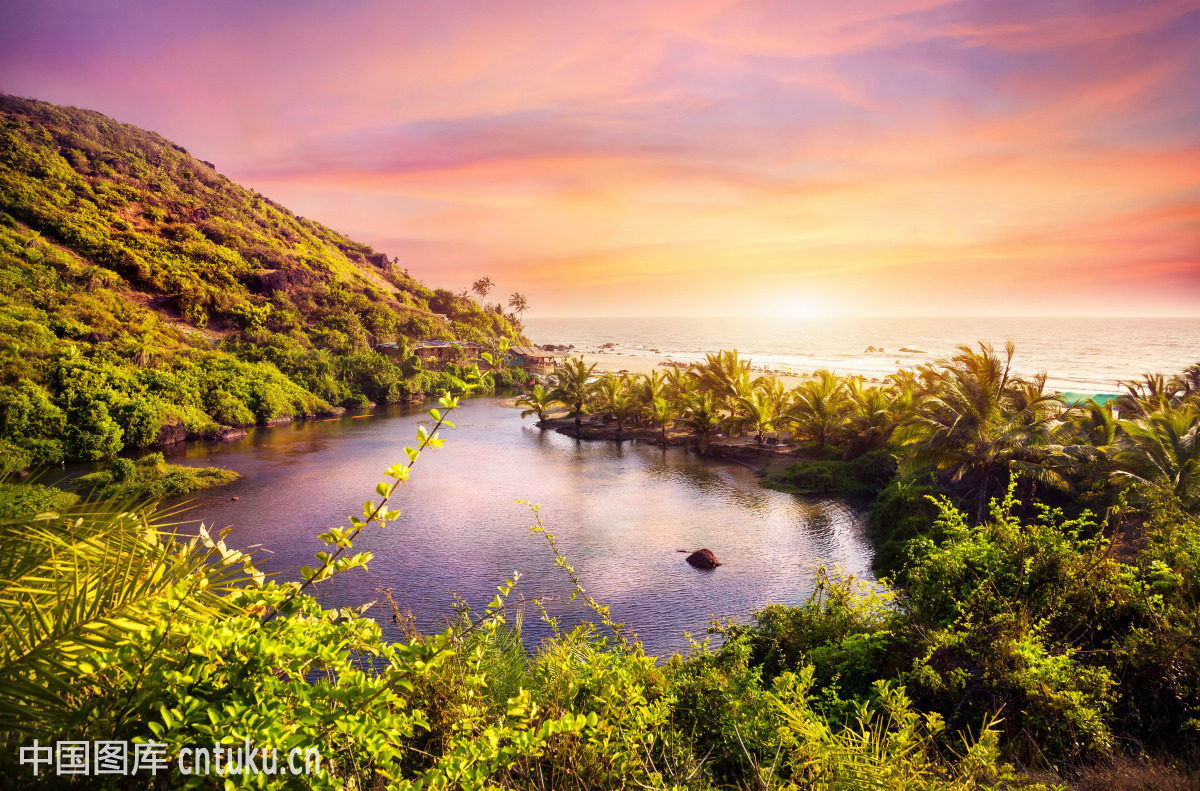
\includegraphics[width=0.6\textwidth]{images/img1.jpg}
		\caption{风景1}\label{fig:s1}
		\end{center}
	\end{figure}
\myfig{风景2}{fig:s2}{0.6}{images/img2.jpg}
  Adobe Photoshop,简称“PS”,是由Adobe Systems开发和发行的图像处理软件。
 Photoshop主要处理以像素所构成的数字图像。使用其众多的编修与绘图工具,可以
 有效地进行图片编辑工作。PS有很多功能,在图像、图形、文字、视频、出版等各方
 面都有涉及。2003年,Adobe Photoshop 8被更名为Adobe Photoshop CS。2013
 年7月,Adobe公司推出了新版本的Photoshop CC,自此,Photoshop CS6作为Adobe
 CS系列的最后一个版本被新的CC系列取代。截止2016年12月Adobe PhotoshopCC2017
 为市场最新版本。如图\ref{fig:s1}所示,又如图\ref{fig:s2}所示。
 {\kaishu 这是楷体吗?}
 
  Adobe Photoshop,简称“PS”,是由Adobe Systems开发和发行的图像处理软件。
 Photoshop主要处理以像素所构成的数字图像。使用其众多的编修与绘图工具,可以
 有效地进行图片编辑工作。PS有很多功能,在图像、图形、文字、视频、出版等各方
 面都有涉及。2003年,Adobe Photoshop 8被更名为Adobe Photoshop CS。2013
 年7月,Adobe公司推出了新版本的Photoshop CC,自此,Photoshop CS6作为Adobe
 CS系列的最后一个版本被新的CC系列取代。截止2016年12月Adobe PhotoshopCC2017
 为市场最新版本。
 {\kaishu 这是楷体吗?}
 
  Adobe Photoshop,简称“PS”,是由Adobe Systems开发和发行的图像处理软件。
 Photoshop主要处理以像素所构成的数字图像。使用其众多的编修与绘图工具,可以
 有效地进行图片编辑工作。PS有很多功能,在图像、图形、文字、视频、出版等各方
 面都有涉及。2003年,Adobe Photoshop 8被更名为Adobe Photoshop CS。2013
 年7月,Adobe公司推出了新版本的Photoshop CC,自此,Photoshop CS6作为Adobe
 CS系列的最后一个版本被新的CC系列取代。截止2016年12月Adobe PhotoshopCC2017
 为市场最新版本。
 {\kaishu 这是楷体吗?}
 
\subsection{phtotshop简介}
 \newpage
	
\mylineskip
\chapter{photoshop基本功能}
\section{phtotshop简介}
Adobe Photoshop,简称“PS”,是由Adobe Systems开发和发行的图像处理软件。
Photoshop主要处理以像素所构成的数字图像。使用其众多的编修与绘图工具,可以
有效地进行图片编辑工作。PS有很多功能,在图像、图形、文字、视频、出版等各方
面都有涉及。2003年,Adobe Photoshop 8被更名为Adobe Photoshop CS。2013
年7月,Adobe公司推出了新版本的Photoshop CC,自此,Photoshop CS6作为Adobe
 CS系列的最后一个版本被新的CC系列取代。截止2016年12月Adobe PhotoshopCC2017
 
 
 Adobe Photoshop,简称“PS”,是由Adobe Systems开发和发行的图像处理软件。
 Photoshop主要处理以像素所构成的数字图像。使用其众多的编修与绘图工具,可以
 有效地进行图片编辑工作。PS有很多功能,在图像、图形、文字、视频、出版等各方
 面都有涉及。2003年,Adobe Photoshop 8被更名为Adobe Photoshop CS。2013
 年7月,Adobe公司推出了新版本的Photoshop CC,自此,Photoshop CS6作为Adobe
 CS系列的最后一个版本被新的CC系列取代。截止2016年12月Adobe PhotoshopCC2017
 为市场最新版本。
 {\kaishu 这是楷体吗?}
 
  Adobe Photoshop,简称“PS”,是由Adobe Systems开发和发行的图像处理软件。
 Photoshop主要处理以像素所构成的数字图像。使用其众多的编修与绘图工具,可以
 有效地进行图片编辑工作。PS有很多功能,在图像、图形、文字、视频、出版等各方
 面都有涉及。2003年,Adobe Photoshop 8被更名为Adobe Photoshop CS。2013
 年7月,Adobe公司推出了新版本的Photoshop CC,自此,Photoshop CS6作为Adobe
 CS系列的最后一个版本被新的CC系列取代。截止2016年12月Adobe PhotoshopCC2017
 为市场最新版本。
 {\kaishu 这是楷体吗?}
 
  Adobe Photoshop,简称“PS”,是由Adobe Systems开发和发行的图像处理软件。
 Photoshop主要处理以像素所构成的数字图像。使用其众多的编修与绘图工具,可以
 有效地进行图片编辑工作。PS有很多功能,在图像、图形、文字、视频、出版等各方
 面都有涉及。2003年,Adobe Photoshop 8被更名为Adobe Photoshop CS。2013
 年7月,Adobe公司推出了新版本的Photoshop CC,自此,Photoshop CS6作为Adobe
 CS系列的最后一个版本被新的CC系列取代。截止2016年12月Adobe PhotoshopCC2017
 为市场最新版本。
 {\kaishu 这是楷体吗?}
 
  Adobe Photoshop,简称“PS”,是由Adobe Systems开发和发行的图像处理软件。
 Photoshop主要处理以像素所构成的数字图像。使用其众多的编修与绘图工具,可以
 有效地进行图片编辑工作。PS有很多功能,在图像、图形、文字、视频、出版等各方
 面都有涉及。2003年,Adobe Photoshop 8被更名为Adobe Photoshop CS。2013
 年7月,Adobe公司推出了新版本的Photoshop CC,自此,Photoshop CS6作为Adobe
 CS系列的最后一个版本被新的CC系列取代。截止2016年12月Adobe PhotoshopCC2017
 为市场最新版本。
 {\kaishu 这是楷体吗?}
 
  Adobe Photoshop,简称“PS”,是由Adobe Systems开发和发行的图像处理软件。
 Photoshop主要处理以像素所构成的数字图像。使用其众多的编修与绘图工具,可以
 有效地进行图片编辑工作。PS有很多功能,在图像、图形、文字、视频、出版等各方
 面都有涉及。2003年,Adobe Photoshop 8被更名为Adobe Photoshop CS。2013
 年7月,Adobe公司推出了新版本的Photoshop CC,自此,Photoshop CS6作为Adobe
 CS系列的最后一个版本被新的CC系列取代。截止2016年12月Adobe PhotoshopCC2017
 为市场最新版本。
 {\kaishu 这是楷体吗?}
 
  Adobe Photoshop,简称“PS”,是由Adobe Systems开发和发行的图像处理软件。
 Photoshop主要处理以像素所构成的数字图像。使用其众多的编修与绘图工具,可以
 有效地进行图片编辑工作。PS有很多功能,在图像、图形、文字、视频、出版等各方
 面都有涉及。2003年,Adobe Photoshop 8被更名为Adobe Photoshop CS。2013
 年7月,Adobe公司推出了新版本的Photoshop CC,自此,Photoshop CS6作为Adobe
 CS系列的最后一个版本被新的CC系列取代。截止2016年12月Adobe PhotoshopCC2017
 为市场最新版本。
 {\kaishu 这是楷体吗?}
 
  Adobe Photoshop,简称“PS”,是由Adobe Systems开发和发行的图像处理软件。
 Photoshop主要处理以像素所构成的数字图像。使用其众多的编修与绘图工具,可以
 有效地进行图片编辑工作。PS有很多功能,在图像、图形、文字、视频、出版等各方
 面都有涉及。2003年,Adobe Photoshop 8被更名为Adobe Photoshop CS。2013
 年7月,Adobe公司推出了新版本的Photoshop CC,自此,Photoshop CS6作为Adobe
 CS系列的最后一个版本被新的CC系列取代。截止2016年12月Adobe PhotoshopCC2017
 为市场最新版本。
 {\kaishu 这是楷体吗?}
 
  Adobe Photoshop,简称“PS”,是由Adobe Systems开发和发行的图像处理软件。
 Photoshop主要处理以像素所构成的数字图像。使用其众多的编修与绘图工具,可以
 有效地进行图片编辑工作。PS有很多功能,在图像、图形、文字、视频、出版等各方
 面都有涉及。2003年,Adobe Photoshop 8被更名为Adobe Photoshop CS。2013
 年7月,Adobe公司推出了新版本的Photoshop CC,自此,Photoshop CS6作为Adobe
 CS系列的最后一个版本被新的CC系列取代。截止2016年12月Adobe PhotoshopCC2017
 为市场最新版本。
 {\kaishu 这是楷体吗?}
 
\subsection{phtotshop简介}
 \newpage
	\backmatter
	
	\appendix
	

\begin{thebibliography}{99}
	\zihao{5}
	\setlength{\itemsep}{-5pt}
	\bibitem{gzp} 广西壮族自治区林业厅. 广西自然保护区[M]. 北京: 中国林业出版社, 1993.
	\bibitem{nue}International Federation of Library Association and Institutions. Names of persons: national usages for entry in catalogues[M]. 3rd ed. London: IFLA International Office for UBC, 1977.
	\bibitem{casc} GANZHA V G, MAYR E W, VOROZHTSOV E V. Computer algebra in scientific computing: CASC 2000: proceedings of the Third Workshop on Computer Algebra in Scientific Computing, Samarkand, October 5-9, 2000[C]. Berlin: Springer, c2000.
\end{thebibliography}
	\chapter{附录}
\section{源代码}
这里是源代码
	\chapter{致谢}
谢谢!
	\chapter{作者简介}
\end{document}